

\subsection{Rutherfords Kernmodell: Das Goldfolienexperiment}
\index{Rutherfords Atommodell}
\index{Goldfolienexperiment}
\index{Atomkern}
\index{Alphateilchen}
\index{Streuung}

Das thomsonsche Atommodell ging davon aus, dass die positive Ladung im Atom
ausgedehnt und gleichmäßig verteilt ist. Die Elektronen waren darin eingebettet.
Dieses Bild wurde durch das Goldfolienexperiment von Ernest Rutherford
grundlegend erschüttert.

Bei diesem Experiment wurden schnelle Alphateilchen auf eine sehr dünne
Goldfolie geschossen. Alphateilchen sind positiv geladene Teilchen. Nach dem
thomsonschen Modell hätte man erwartet, dass diese Teilchen die Goldfolie fast
ungehindert durchqueren und höchstens leicht abgelenkt werden. Eine ausgedehnte,
gleichmäßig verteilte positive Ladung hätte keine starke punktartige Abstoßung
verursachen können.

Die Beobachtung war jedoch überraschend. Die meisten Alphateilchen gingen
tatsächlich nahezu gerade durch die Folie hindurch. Einige wenige wurden aber
stark abgelenkt, und ein sehr kleiner Anteil wurde sogar zurückgestreut. Das
war mit dem Rosinenkuchenmodell nicht erklärbar.

Rutherford schloss daraus, dass die positive Ladung und fast die gesamte Masse
des Atoms in einem sehr kleinen Bereich konzentriert sein müssen. Diesen Bereich
bezeichnet man als Atomkern. Das Atom besteht demnach größtenteils aus leerem
Raum. Die Elektronen befinden sich außerhalb des Kerns.
\FloatBarrier
\begin{figure}[H]
	\centering
	 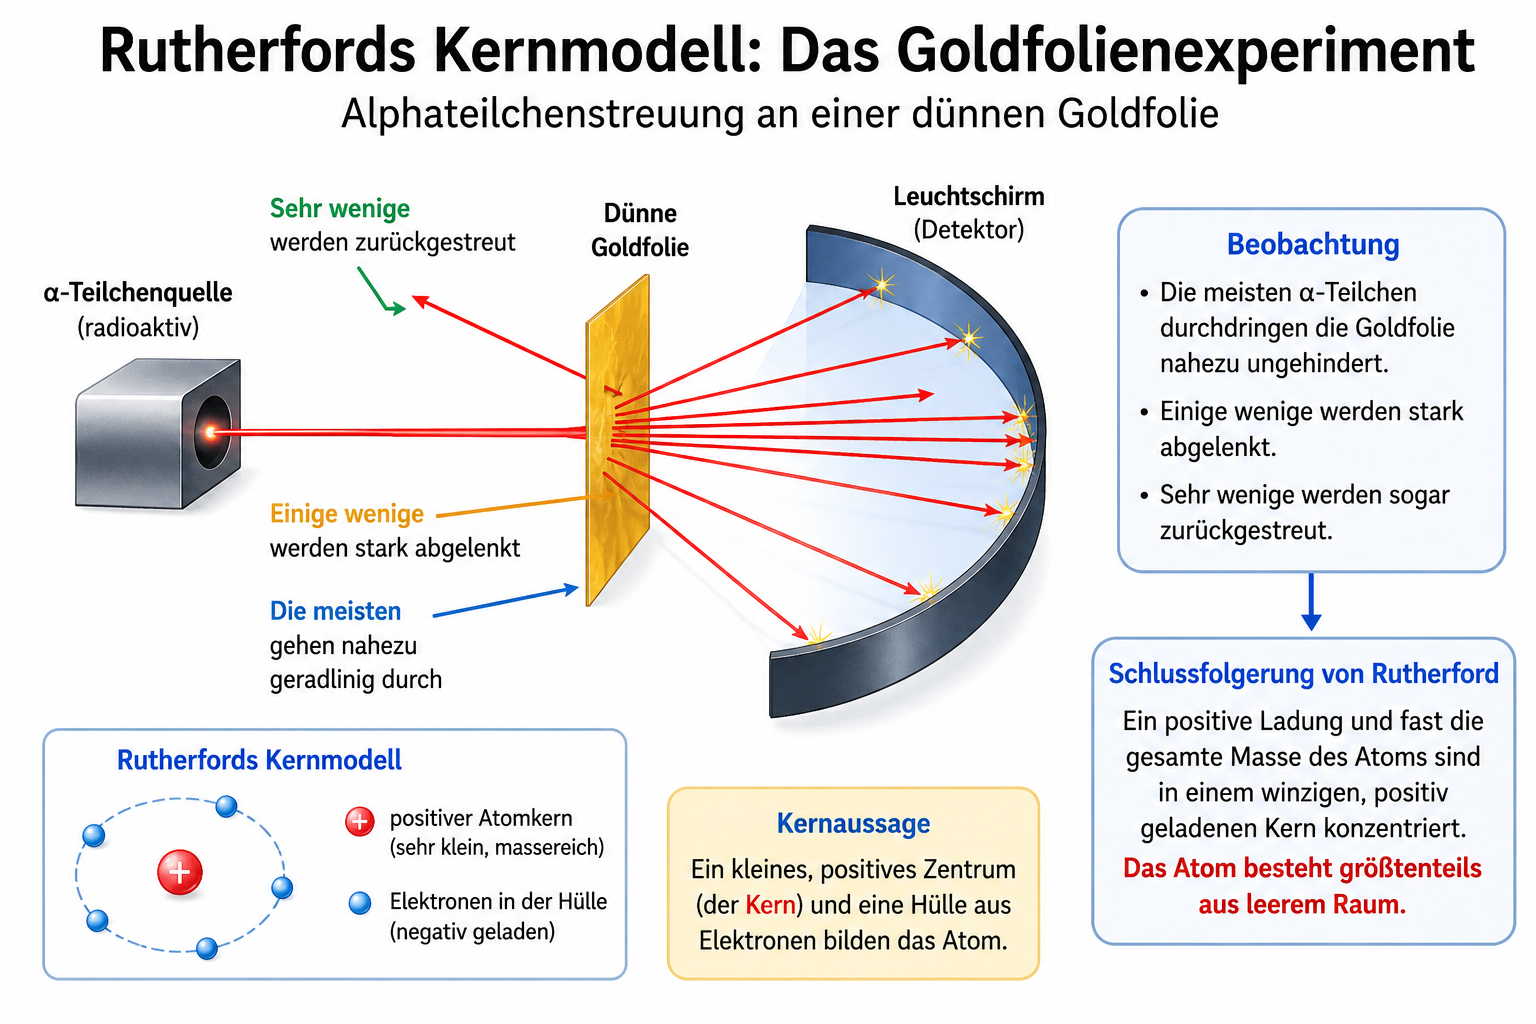
\includegraphics[width=0.75\textwidth]{bilder/goldfolie}
	\caption{Schematische Darstellung des Goldfolienexperiments. Die meisten
		Alphateilchen durchdringen die Goldfolie nahezu geradlinig. Einige wenige
		werden stark abgelenkt oder zurückgestreut. Daraus folgerte Rutherford die
		Existenz eines kleinen, positiv geladenen Atomkerns.}
	\label{fig:rutherford_goldfolienexperiment}
\end{figure}

Damit entstand ein neues Atommodell: das Kern-Hülle-Modell. Im Zentrum befindet
sich der kleine, positiv geladene Atomkern. Die negativ geladenen Elektronen
bilden die äußere Hülle. Die elektrische Anziehung zwischen Kern und Elektronen
hält das Atom zusammen.

Dieses Modell war ein gewaltiger Fortschritt. Es erklärte, warum die meisten
Alphateilchen ungehindert durch die Goldfolie laufen: Sie bewegen sich durch
den fast leeren Raum zwischen den Atomkernen. Es erklärte auch, warum einige
wenige Alphateilchen stark abgelenkt werden: Sie kommen dem kleinen, positiv
geladenen Kern sehr nahe und werden durch die elektrische Abstoßung abgelenkt.

Für das Elektron bedeutete Rutherfords Modell eine neue Rolle. Es war nicht mehr
einfach in eine positive Ladungsmasse eingebettet, sondern Teil einer Hülle um
einen zentralen Kern. Damit wurde das Atom erstmals als System aus Kern und
Elektronenhülle verstanden.

Allerdings hatte dieses Modell ein schwerwiegendes Problem. Nach der klassischen
Elektrodynamik müsste ein Elektron, das sich um den positiv geladenen Kern
bewegt, elektromagnetische Strahlung aussenden. Dabei würde es Energie verlieren
und in kurzer Zeit in den Kern stürzen. Klassisch wäre ein solches Atom also
nicht stabil.

Die Stabilität der Atome konnte Rutherfords Modell daher noch nicht erklären.
Genau an dieser Stelle wurde der nächste Schritt notwendig: das bohrsche
Atommodell mit quantisierten Elektronenbahnen.

\begin{PhysicsBox}[Rutherfords Kernaussage]
	
	\label{box:rutherford-kernaussage}
	Das Goldfolienexperiment zeigte, dass die positive Ladung und fast die gesamte
	Masse des Atoms in einem winzigen Atomkern konzentriert sind.
	
	Die meisten Alphateilchen durchdringen die Goldfolie nahezu geradlinig, weil
	das Atom größtenteils aus leerem Raum besteht. Starke Ablenkungen entstehen nur,
	wenn ein Alphateilchen dem kleinen, positiv geladenen Kern sehr nahe kommt.
	
\end{PhysicsBox}